\label{sec:intro}

La utilización de imágenes satelitales permite analizar grandes extensiones del
territorio, contando con un registro histórico con el cual realizar
comparaciones.

En la provincia de Misiones, el departamento de Iguaz\'u es lindante a Brasil y
Paraguay siendo parte de la zona conocida como triple frontera
perteneciente a la ecorregi\'on conocida como \emph{selva paranaense} (Figura \ref{parque}). All\'i podemos encontrar Represa de Urugua-\'{\i} y el Parque Nacional
Iguaz\'u. El departamento tiene un area de $2.736 km^2$ y una poblaci\'on de
$82.227$ seg\'un el \'ultimo senso del INDEC.

\begin{figure}[h!]
  \centering
  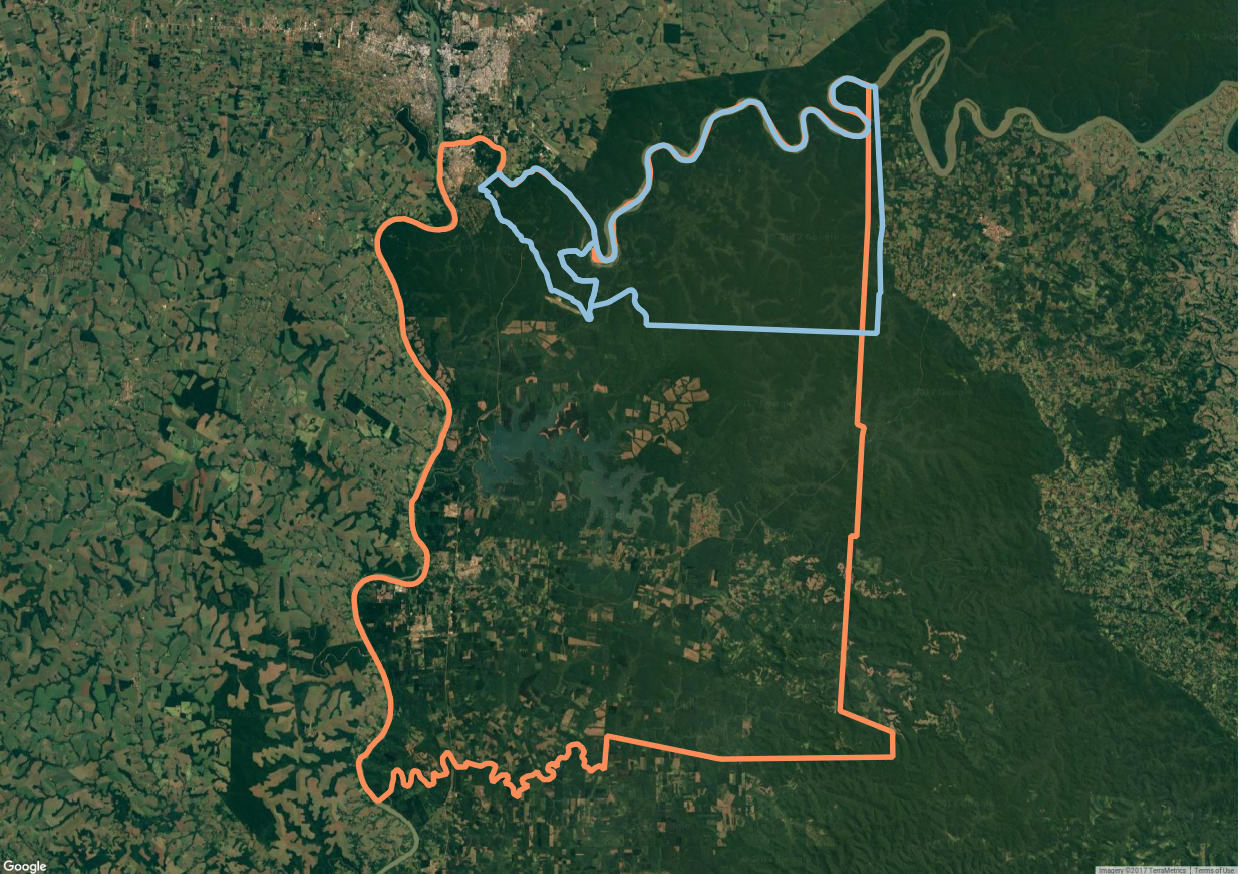
\includegraphics[width=0.8\textwidth]{triple.png}
  \caption{Departamento de Iguaz\'u, en rosa, y parque natural Iguaz\'u, en celeste.}
  \label{parque}
\end{figure}

Tomaremos al departamento como \'area de estudio durante este curso
con el objetivo de obtener un mapa de uso y cobertura que nos
permita estimar y validar sus superficies.

Utilizaremos imagenes de los satelites Landsat 8, Landsat 7 y
el producto de MOD13Q1 obtenido de los satelites TERRA y AQUA durante
el periodo 2000-2016.

\section{Organizacion del curso}

El curso se divide en dos partes. En la primera trabajaremos con la compresi\'on
del espacio espectral y el uso de las im\'agenes satelitales para extraer valores continuos de las variables biof\'isicas.

Cap\'itulo  \ref{viaje}, \nameref{viaje}, estudiaremos las firmas espectrales de
distintas coberturas y como se relacionan con las propiedades biofisicas.
Introduciremos el concepto de espacio espectral como el
lugar natural donde realizar el an\'alisis en teledetecci\'on.

Cap\'itulo  \ref{rebotando}, \nameref{rebotando}, estudiaremos distintas
formas de obtener la reflectancia de las coberturas a partir de los datos satelitales. Analizaremos m\'etodos de correcci\'on atmosf\'erica basados en propiedades estad\'isticas de las im\'agenes y en el modelado de la atm\'osfera.

Cap\'itulo  \ref{abaco}, \nameref{abaco}, veremos como a partir de los valores de reflectancia para una cobertura y operaciones matem\'aticas, podemos obtener los valores de variables biof\'isicas continuas como son el contenido de clorofila o humedad.

Cap\'itulo  \ref{rotaciones}, \nameref{rotaciones}, empezaremos a utilizar herramientas geom\'etricas en el espacio espectral para resaltar distintas propiedades de las im\'agenes y poner en evidencia cuales son las zonas del espectro que m\'as informaci\'on aportan sobre nuesta zona de estudio.

En la segunda parte del curso trabajaremos m\'as en detalle con el espacio
espectral usando sus propiedades para extraer informaci\'on categ\'orica de
las im\'agenes.

Cap\'itulo  \ref{otrolado}, \nameref{otrolado}, veremos como utilizar herramientas que no requieren de conocimiento previo del \'area de estudio para realizar segmentaciones en el espacio de fases de la imagen y obtener mapas de uso y cobertura.

Cap\'itulo  \ref{educando}, \nameref{educando}, veremos otros m\'etodos para extraer informaci\'on categ\'orica sobre las im\'agenes satelitales al estudiar distintas formas de clasificaci\'on supervisada.

Cap\'itulo  \ref{pos}, \nameref{pos}, veremos algunas t\'ecnicas de postprocesamiento que nos permitiran analizar el contexto espacial de nuestras clasificaciones y calcular superficies de coberturas para las im\'agenes y su correspondiente incerteza.

Puede consultar el cronograma detallado en el apendice \ref{chap:cronograma}.

\subsection{Forma de aprobaci\'on}
Para aprobar el curso se deben reunior al menos 100 puntos entre las distintas actividades. Adem\'a deberan completarse dos cuestionarios \emph{obligatorios} al comenzar y finalizar el curso.

La nota final del curso estara dada por el siguiente rango

\begin{itemize}
\item 0 - 99 - No aprobó
\item 100-109 - Seis
\item 110-129 - Siete
\item 130-169 - Ocho
\item 170-189 - Nueve
\item 190-200 - Diez
\end{itemize}

Los puntos se determinan de la siguiente manera

\begin{itemize}
  \item Cada cuestionario: 0 a 10 puntos. Máximo 70.
  \item Cada tarea: 0 a 50 puntos. Máximo 100.
  \item Participar en la plataforma: 0 a 10 puntos. Sin máximo.
\end{itemize}

\section{Material del curso}
Todo el material del curso se encuentra disponible para descargar en el aula virtual del curso. Est\'a organizado de la siguiente manera

\dirtree{%
    .1 material.
    .2 aux\_data.
    .2 example\_scripts.
    .2 raster\_data.
    .2 vector\_data.
    }

conteniendo la carpeta \file{aux\_data} archivos adicionales para trabajar, \file{example\_scripts} todos los scripts que se encuentran en esta guia, \file{raster\_data} los archivos raster cada uno en una carpeta y \file{vector\_data} los archivos vectoriales para usar durante el curso.

Todos los materiales del curso, con sus correspondientes editables, pueden
encontrarse en el repositorio de github \url{https://github.com/fnemina/curso-sopi-herramientas-cuantitativas}.
